%---------- Inleiding ---------------------------------------------------------

\section{Introductie}%
\label{sec:introductie}

De bachelorproef zal zich focussen op de evoluerende complexiteit van moderne bedrijfsapplicaties en de architecturale benaderingen die worden ingezet om aan deze groeiende behoeften te voldoen. Het kernthema van mijn onderzoek betreft de keuze tussen een monolithische architectuur en een microservices architectuur bij de ontwikkeling van bedrijfsapplicaties. Deze keuze wordt steeds relevanter vanwege de voortdurende toename en verandering van de complexiteit waarmee ondernemingen te maken hebben. Bedrijven overwegen vaak om de stabiliteit van een monolithische softwarearchitectuur los te laten en te opteren voor een servicegerichte architectuur. Het onderzoek is gedreven door de noodzaak van flexibiliteit in softwarearchitecturen, en daarom wordt de beweging van veel bedrijven om over te stappen van een monolithische naar een servicegerichte aanpak nauwgezet onderzocht. Het centrale thema van de bachelorproef is de vergelijking tussen beide architecturen, waarbij specifieke aandacht wordt besteed aan de voor- en nadelen van elk. De verschuiving naar een servicegerichte benadering wordt verder onderzocht met als doel richtlijnen te ontwikkelen voor bedrijven die deze overgang overwegen. Dit onderzoek wordt concreet toegepast in een casestudy over software in een dierenkliniek, waarmee praktische inzichten worden verkregen die relevant zijn voor de bredere context van bedrijfsapplicatieontwikkeling.

In het kader van deze studie zal ik me specifiek richten op een dierenkliniekapplicatie, die zal eerst opgezet worden als een monolithische architectuur met behulp van Spring Boot. Deze applicatie omvat diverse functionaliteiten, zoals het beheer van klanten, dieren en artsen, het maken van afspraken, het registreren van prestaties, het aanmaken en verzenden van facturen, en het volgen van betalingen.

Het onderzoek heeft als doel inzicht te bieden in de mogelijkheden van schaalbaarheid en prestatieverbetering door de overstap naar een microservices architectuur in combinatie met een servicemesh. Hierbij zal ik de functionaliteiten van de applicatie opdelen in verschillende microservices, zoals CRM, beheer van afspraken, beheer van prestaties, facturatie en betalingen. Deze microservices zullen vervolgens worden beheerd en met elkaar communiceren via een servicemesh.

Om dit doel te bereiken, zal ik me richten op de volgende aspecten:

Kaderen van het thema: Het onderzoek zal de overstap van een monolithische naar een microservices architectuur in de context van bedrijfsapplicaties belichten, met bijzondere aandacht voor de dierenkliniekapplicatie.

Doelgroep: De doelgroep van dit onderzoek zijn ontwikkelaars, architecten en besluitvormers die betrokken zijn bij de bouw en evolutie van bedrijfsapplicaties.

Probleemstelling en (centrale) onderzoeksvraag: De huidige monolithische architectuur van de dierenkliniekapplicatie roept vragen op over schaalbaarheid en prestaties. De centrale onderzoeksvraag luidt: "Hoe kan de dierenkliniekapplicatie profiteren van een microservices architectuur in combinatie met een servicemesh om schaalbaarheid en prestaties te verbeteren?"

Onderzoeksdoelstelling: Het onderzoek streeft ernaar inzicht te verschaffen in de architecturale overwegingen en best practices bij het gebruik van een servicemesh voor schaalbaarheid en prestatieverbetering in bedrijfsapplicaties, met de dierenkliniekapplicatie als specifieke case study.

In de vervolgstappen van dit onderzoeksvoorstel zal ik dieper ingaan op relevante literatuur, de toegepaste methodologie, en de verwachte resultaten en conclusies die ik hoop te verkrijgen.
%---------- Stand van zaken ---------------------------------------------------

\section{State-of-the-art}%
\label{sec:state-of-the-art}

We kunnen de vergelijking maken  tussen monolithische en microservices architectuur. Een monolithische architectuur bestaat uit één codebase met alle functionaliteit, terwijl een \linebreak microservices architectuur gebruik maakt van onafhankelijke services. Microservices bieden flexibiliteit en schaalbaarheid, maar brengen ook complexiteit met zich mee, zoals service discovery en monitoring. De juiste architectuurkeuze hangt af van de behoeften en complexiteit van het project.

Deze adoptie van microservices architectuur heeft geleid tot de opkomst van servicemeshes als een mechanisme voor het beheren van de communicatie en interactie tussen de verschillende services binnen een applicatie. Een servicemesh is een abstractielaag die een reeks functies biedt, zoals load balancing, service discovery, monitoring en beveiliging, die essentieel zijn voor het schalen en beheren van microservices.

% Voor literatuurverwijzingen zijn er twee belangrijke commando's:
% \autocite{KEY} => (Auteur, jaartal) Gebruik dit als de naam van de auteur
%   geen onderdeel is van de zin.
% \textcite{KEY} => Auteur (jaartal)  Gebruik dit als de auteursnaam wel een
%   functie heeft in de zin (bv. ``Uit onderzoek door Doll & Hill (1954) bleek
%   ...'')


\section{Literatuuronderzoek}
\label{sec:literatuuronderzoek}
Voor er een vergelijking kan gemaakt worden tussen monolithische en microservices architectuur moeten we eerst eens terug kijken naar hoe deze twee architecturen zich tot elkaar verhouden.


\subsection*{Monolithische architectuur}
Laten we beginnen met monolithische applicaties, hoewel ze enkele voordelen bieden, worden vaak geconfronteerd met aanzienlijke nadelen die van invloed kunnen zijn op de ontwikkeling, schaalbaarheid en onderhoud van de software. 
Een van de belangrijkste nadelen is de groeiende complexiteit van de codebase naarmate de applicatie evolueert. Deze toenemende complexiteit kan leiden tot overbelasting van de ontwikkelomgeving, waardoor de productiviteit van ontwikkelaars afneemt. Het veranderen van de technologiestack van de applicatie kan een uitdagende taak zijn, en het herstructureren van de codebase wordt bemoeilijkt door de onvoorspelbare impact op de applicatiefunctionaliteit. 
Een kritiek punt is het risico van volledige uitval wanneer een enkele functie of component van de applicatie faalt. Bovendien neemt de kwaliteit van een monolithische architectuur geleidelijk af in de loop van de tijd door de constante toevoeging van nieuwe componenten, wat resulteert in een afname van de verwerkingssnelheid.
De architectuur wordt ook als veeleisend ervaren om te begrijpen, vooral naarmate de codebase groeit. Dit vereist meestal een diepgaande kennis van het gehele systeem. Nieuwe ontwikkelaars hebben moeite om veranderingen in de volledige codebase te begrijpen, zelfs met gedetailleerde documentatie. Schaalbaarheidsproblemen, uitdagend onderhoud en moeilijkheden bij het upgraden van de applicatie vormen verdere obstakels. 
Desondanks hebben monolithische applicaties enkele voordelen. Ze zijn eenvoudig te ontwikkelen, gemakkelijk te debuggen en niet veeleisend om op te zetten. Vooral geschikt voor kleine projecten, zoals MVP's of proof of concepts, bieden ze een eenvoudig te gebruiken en aanpasbaar ecosysteem. In situaties waar schaalvergroting niet nodig is, kunnen monolithische architecturen de benodigde oplossing bieden. Bovendien ervaren ze minder netwerkproblemen in vergelijking met microservices. Het is echter van cruciaal belang om deze voordelen af te wegen tegen de ernstige nadelen bij het kiezen van de juiste architectuur voor een specifieke toepassing.

\begin{figure}[h]
	\centering	
	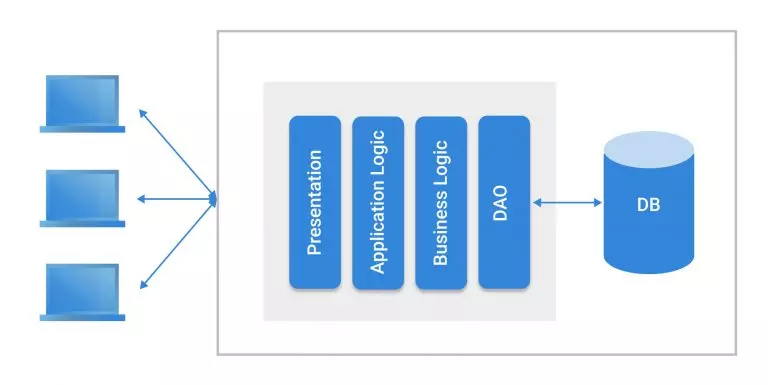
\includegraphics[width = 9cm]{MonolithicImage1.png} 
	\caption{Monoliet} 
	\label{fig:Monoliet} 
\end{figure}
\FloatBarrier

\subsection*{Microservices architectuur}
Dan hebben we microservices-architecturen die een manier zijn  om grote softwareprojecten op te splitsen in losjes gekoppelde modules, die met elkaar communiceren via eenvoudige Application Programming Interfaces (API's). Volgens Adrian Cockcroft, voorheen werkzaam bij Netflix, is "Een microservices-architectuur een servicegerichte architectuur, samengesteld uit losjes gekoppelde elementen met begrensde contexten " (vertaald vanuit het Engels) ~\autocite{Richardson2018}.

Microservices bieden diverse voordelen die gericht zijn op flexibiliteit, schaalbaarheid en foutisolatie. Eén van de belangrijkste voordelen is de mogelijkheid om onafhankelijke, herbruikbare componenten te creëren. Deze componenten kunnen afzonderlijk worden geïmplementeerd in andere applicaties zonder invloed op andere eenheden. Het modulaire karakter van microservices maakt het eenvoudig te debuggen, schalen en begrijpen, wat bijdraagt aan een snellere ontwikkeling en implementatie. 
Microservices stellen ontwikkelaars in staat om specifieke componenten te schalen of ongewijzigd te laten, waardoor een hoog niveau van flexibiliteit ontstaat. Verbeterde foutisolatie is ook een voordeel, omdat falen in één module de prestaties van de gehele applicatie niet significant beïnvloedt. Daarnaast biedt de mogelijkheid om nieuwe technologieën toe te voegen en te testen, evenals het elimineren van leverancier- of technologielock-in, extra voordelen voor wendbaarheid en innovatie. 

Aan de andere kant zijn er ook nadelen verbonden aan microservices. De architectuur kan te ingewikkeld worden naarmate het systeem groeit, waardoor het beheer bemoeilijkt wordt. Het testen kan veeleisend zijn, vooral bij complexe systemen, en het onderhoud kan duurder worden naarmate meer eenheden worden toegevoegd. Beveiligingsproblemen zijn een zorg, aangezien de gedistribueerde aard van microservices verschillende faalpunten introduceert. 
De complexiteit van communicatie tussen services, de kosten van individuele servers en databases voor elke microservice, en de kwetsbaarheid voor beveiligingsproblemen zijn belangrijke nadelen. Ook brengt de complexiteit van coördinatie tussen services uitdagingen met zich mee bij implementatie, vooral voor kleine bedrijven die snel willen creëren en itereren. Het testen van microservices-gebaseerde applicaties kan omslachtig zijn, en het opsporen van fouten vereist grondig doorzoeken van de logboeken van elke service. 
Hoewel microservices veel voordelen bieden, moeten organisaties zorgvuldig afwegen of de voordelen opwegen tegen de complexiteit en uitdagingen die de implementatie van deze architectuur met zich meebrengt.

\begin{figure}[h]
	\centering	
	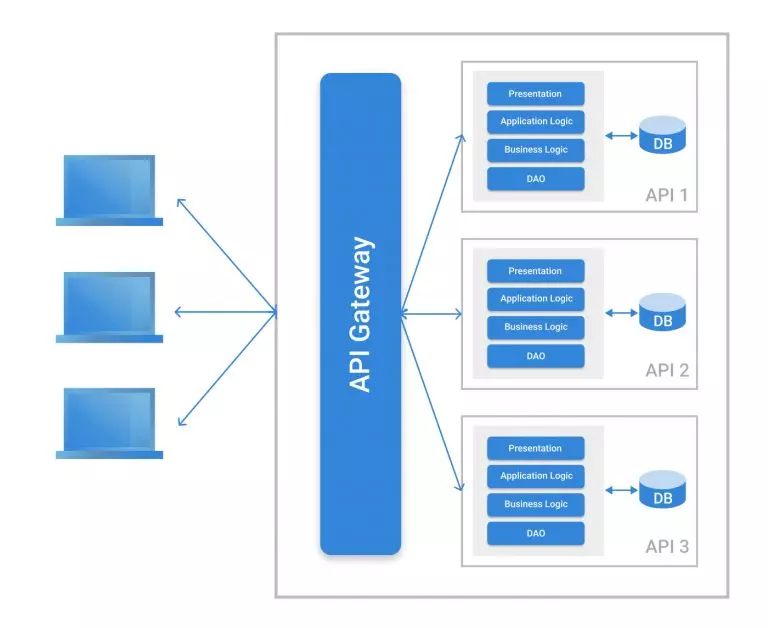
\includegraphics[width = 9cm]{MicroserviceImage1.png} 
	\caption{Microservice} 
	\label{fig:Microservice} 
\end{figure}
\FloatBarrier

\subsection*{Lehman's wetten van software-evolutie}
Al lang voor het ontstaan van microservice kwam Lehman met zijn acht wetten van software-evolutie. Deze wetten beschrijven de dynamiek van softwaresystemen over tijd en benadrukken de noodzaak van voortdurende aanpassing aan nieuwe behoeften, beheersing van toenemende complexiteit, en behoud van stabiliteit en bekendheid. Het behoud van organisatorische stabiliteit en bekendheid, gecombineerd met voortdurende groei in functionaliteit, vormt de kern van Lehman's inzichten. Tevens waarschuwen de wetten voor mogelijke afname in kwaliteit over tijd, waarbij een feedbacksysteem cruciaal is voor een succesvolle evolutie, met erkenning van de rol van gebruikersfeedback in het stimuleren van toekomstige ontwikkelingen.

\begin{enumerate}
	\item \textbf{Continuing Change:} Lehman stelt dat een softwaresysteem in de loop der tijd steeds minder bevredigend wordt voor gebruikers, tenzij het voortdurend wordt aangepast aan nieuwe behoeften. De noodzaak van voortdurende aanpassing staat hierbij centraal.
	
	\item \textbf{Increasing Complexity:} Softwaresystemen worden volgens Lehman steeds complexer, tenzij actieve inspanningen worden geleverd om deze complexiteit te verminderen. Deze wet benadrukt de essentie van proactieve maatregelen om de inherente neiging tot complexiteitsgroei te beheersen.
	
	\item \textbf{Self-Regulation:} Het proces van software-evolutie reguleert volgens Lehman zichzelf, met een distributie van product- en procesartefacten die dicht bij normaal ligt. Dit impliceert een natuurlijk evenwicht in het evolutieproces, in lijn met typische statistische patronen.
	
	\item \textbf{Conservation of Organizational Stability:} Het gemiddelde effectieve wereldwijde activiteitsniveau op een evoluerend softwaresysteem verandert niet in de loop der tijd. Dit suggereert dat de hoeveelheid werk in elke release volgens Lehman relatief constant blijft en bijdraagt aan de stabiliteit van het ontwikkelingsproces.
	
	\item \textbf{Conservation of Familiarity:} De hoeveelheid nieuwe inhoud in opeenvolgende releases neigt constant te blijven of af te nemen. Deze wet belicht de trend om het behoud of de vermindering van de introductie van nieuwe elementen in software-releases.
	
	\item \textbf{Continuing Growth:} De hoeveelheid functionaliteit in een softwaresysteem zal toenemen om aan de verwachtingen van gebruikers te voldoen. Dit erkent de noodzaak om de mogelijkheden van software te verbeteren voor voortdurende relevantie en bruikbaarheid.
	
	\item \textbf{Declining Quality:} Een softwaresysteem wordt gezien als afnemend in kwaliteit, tenzij het ontwerp zorgvuldig wordt onderhouden en aangepast aan nieuwe operationele beperkingen. Dit onderstreept het belang van continue kwaliteitsborging en ontwerpoverwegingen.
	
	\item \textbf{Feedback System:} Het succesvol evolueren van een softwaresysteem vereist erkenning van het ontwikkelingsproces als een multi-loop, multi-agent, multi-level feedbacksysteem. Naarmate een softwaresysteem ouder wordt, wordt het steeds moeilijker te veranderen vanwege de complexiteit van zowel artefacten als processen, waarbij de rol van gebruikersfeedback in de toekomstige evolutie wordt erkend. ~\autocite{Godfrey2013}
\end{enumerate}

\subsection*{Ontstaan van Microservices}
Microservices zijn ontstaan uit frustraties met traditionele monolithische architectuur. Deze benadering omvat het bouwen van applicaties als suites van onafhankelijke, schaalbare services. Elke service heeft een duidelijke modulegrens, waardoor ze zelfs in verschillende programmeertalen kunnen worden geschreven en door verschillende teams kunnen worden beheerd. De microservices-stijl is niets nieuws. De oorsprong gaat terug tot Unix-ontwerpprincipes. Hoewel er geen formele definitie bestaat, delen microservice-architecturen gemeenschappelijke kenmerken die bijdragen aan hun flexibiliteit en schaalbaarheid. ~\autocite{Fowler2014}.

\begin{enumerate}
	\item \textbf{Componentization via Services:} Microservices worden behandeld als onafhankelijke componenten die afzonderlijk kunnen worden geïmplementeerd en bijgewerkt.
	
	\item \textbf{Organized around Business Capabilities:} Microservices zijn georganiseerd rond zakelijke mogelijkheden, wat betekent dat elke service overeenkomt met een zakelijke functionaliteit.
	
	\item \textbf{Products not Projects:} teams bezitten een bepaald product gedurende de volledige levensduur ervan, in plaats van alleen maar aan projecten te werken.
	
	\item \textbf{Smart endpoints and dumb pipes:} Applicaties die zijn opgebouwd uit microservices streven ernaar zo ontkoppeld en samenhangend mogelijk te zijn. Ze communiceren met elkaar via eenvoudige API’s, terwijl ze de onderliggende communicatie-complexiteit \linebreak  weghouden van de services. 
	
	\item \textbf{Decentralized Governance:} Verschillende diensten kunnen verschillende technologieën gebruiken (programmeertalen, databases, enz.). Er is geen gestandaardiseerd mandaat voor alle diensten.
	
	\item \textbf{Decentralized Data Management:} Elke dienst heeft zijn eigen database om de ontkoppeling van andere diensten te garanderen.
	
	\item \textbf{Infrastructure Automation:} gebruik van continue integratie en continue implementatie om de services te beheren.
	
	\item \textbf{Design for failure:} Diensten moeten worden ontworpen met het oog op het feit dat ze zullen mislukken. Dit helpt bij het bouwen van veerkrachtige systemen.
	
	\item \textbf{Evolutionary Design:} Het is de bedoeling dat het systeemontwerp in de loop van de tijd evolueert, en nieuwe technologieën en praktijken kunnen worden toegepast wanneer dat nodig is. ~\autocite{Fowler2014}.
\end{enumerate}

\subsection*{Servicemeshes}
Deze adoptie van microservices architectuur heeft geleid tot de opkomst van servicemeshes als een mechanisme voor het beheren van de communicatie en interactie tussen de verschillende services binnen een applicatie. Een servicemesh is een abstractielaag die een reeks functies biedt, zoals load balancing, service discovery, monitoring en beveiliging, die essentieel zijn voor het schalen en beheren van microservices.

Een belangrijke architecturale overweging bij het gebruik van een servicemesh is service discovery. In tegenstelling tot een monolithische architectuur, waarbij functionaliteiten vaak hardgecodeerde afhankelijkheden hebben, maakt een servicemesh gebruik van dynamische service discovery. Dit stelt services in staat om automatisch nieuwe services te ontdekken en ermee te communiceren zonder handmatige configuratiewijzigingen. Een voorbeeld van een servicemesh implementatie die service discovery mogelijk maakt, is Istio ~\autocite{Morgan2021}.

Een andere belangrijk aspect is load balancing. Een servicemesh verdeelt het verkeer gelijkmatig over de beschikbare service instances, waardoor de prestaties worden geoptimaliseerd, de belasting op afzonderlijke instances onder controle blijft en er ad hoc extra instances kunnen opgespind worden. Dit is vooral nuttig in bedrijfsapplicaties waar veel services parallel moeten worden geschaald om aan de vraag te voldoen ~\autocite{Ciobotaru2020}.

Monitoring en tracing van service traffic zijn ook cruciale aspecten bij het gebruik van een servicemesh. Door het instrumenteren van services met monitoring- en tracingfunctionaliteit, kan een servicemesh gedetailleerd inzicht bieden in de prestaties en het gedrag van services. Dit is met name waardevol in bedrijfsapplicaties waar de complexiteit van de interacties tussen services kan leiden tot moeilijkheden bij het identificeren en oplossen van problemen \linebreak ~\autocite{Ciobotaru2021}.

Servicemeshes verhogen de weerbaarheid door het implementeren van verschillende resilience patterns. Hierdoor kan tijdelijke onbeschikbaarheid of overbelasting van services opgevangen worden.

\subsection*{Kort samengevat}

Een monolithische architectuur biedt eenvoud en een eenvoudige implementatie, maar kan het uitdagend zijn bij groei. Microservices bieden flexibiliteit en schaalbaarheid, maar kunnen complexer en duurder zijn in onderhoud.

Een monolithische architectuur bestaat uit één codebase met alle functionaliteit, terwijl een \linebreak microservices architectuur gebruik maakt van onafhankelijke services. Microservices bieden flexibiliteit en schaalbaarheid, maar brengen ook complexiteit met zich mee, zoals service discovery en monitoring. De juiste architectuurkeuze hangt af van de behoeften en complexiteit van het project.

Lehman's acht wetten van software-evolutie schetsen de dynamiek van softwaresystemen in de loop van de tijd. Ze onderstrepen de noodzaak van voortdurende aanpassing aan nieuwe behoeften, het beheersen van toenemende complexiteit, en het handhaven van evenwicht in het evolutieproces. Het behoud van organisatorische stabiliteit en vertrouwdheid, tezamen met voortdurende groei in functionaliteit, vormt de kern van Lehman's inzichten. Tegelijkertijd waarschuwen de wetten voor mogelijke afname in kwaliteit na verloop van tijd, waarbij een feedbacksysteem cruciaal is voor een succesvolle evolutie, met erkenning van de rol van gebruikersfeedback in het stimuleren van toekomstige ontwikkelingen. 

Lehman's wetten vinden dus toepassing in zowel monolithische als gedistribueerde (microservices) systemen. In het geval van monolithische architecturen benadrukken deze wetten de noodzaak van voortdurende aanpassing aan veranderende eisen, beheersing van complexiteit, en behoud van stabiliteit en bekendheid. 

De vraag rijst echter of Microservices een oplossing kunnen bieden voor enkele uitdagingen die voortvloeien uit Lehman's wetten.


\section{Opzetten van de Architectuur}
\label{sec:architectuur}
Voor de implementatie van mijn microservices heb ik gekozen voor Istio. Om vertrouwd te raken met dit hulpmiddel, ben ik begonnen met het opzetten van een eenvoudige microservice die gebruikmaakt van voorbeeldgegevens.

De eerste stap was het downloaden van Istio. Dit kan worden gedaan door de volgende opdrachten uit te voeren:

\begin{lstlisting}[language=bash]
$ curl -L https://istio.io/downloadIstio | sh -
$ cd istio-1.21.1
$ export PATH=$PWD/bin:$PATH
\end{lstlisting}

Nadat dit is voltooid, kan Istio worden geïnstalleerd met het volgende commando:

\begin{lstlisting}[language=bash]
$ istioctl install --set profile=demo -y
\end{lstlisting}

Voordat u dit commando uitvoert, moet u echter eerst een Kubernetes-cluster hebben opgezet. Als u nog geen Kubernetes heeft geïnstalleerd, kunt u dit doen met het volgende commando:

\begin{lstlisting}[language=bash]
$ brew install kubectl
\end{lstlisting}

Dit kan worden gedaan met behulp van Minikube en Hyperkit. De installatie van Minikube en Hyperkit kan worden uitgevoerd met de volgende commando's:

\begin{lstlisting}[language=bash]
$ brew install minikube
$ brew install hyperkit
\end{lstlisting}

Als Minikube en Hyperkit zijn geïnstalleerd, kunt u een cluster opzetten met het volgende commando:

\begin{lstlisting}[language=bash]
$ minikube start --driver=hyperkit
\end{lstlisting}

Nadat u dit heeft gedaan, kunt u Istio installeren met het eerder genoemde commando. Als laatste stap moet u nog de Istio sidecar-injectie inschakelen met het commando:

\begin{lstlisting}[language=bash]
$ kubectl label namespace default istio-injection=enabled
\end{lstlisting}

Vervolgens heb ik de voorbeeldapplicatie gedeployed met het volgende commando:

\begin{lstlisting}[language=bash]
$ kubectl apply -f samples/bookinfo/platform/kube/bookinfo.yaml
\end{lstlisting}

Zorg ervoor dat alle pods en services actief zijn door de volgende commando's uit te voeren:

\begin{lstlisting}[language=bash]
$ kubectl get services
$ kubectl get pods
\end{lstlisting}

De volgende stap is het verbinden met een Istio gateway. Dit kan worden gedaan met het commando:

\begin{lstlisting}[language=bash]
$ kubectl apply -f samples/bookinfo/networking/bookinfo-gateway.yaml
\end{lstlisting}

Dit kunt u controleren met het \verb|istioctl analyze| commando. Vervolgens moeten de ingress host en poort worden ingesteld. Dit heb ik gedaan door eerst het \verb|minikube tunnel| commando uit te voeren en vervolgens de volgende commando's uit te voeren:

\begin{lstlisting}[language=bash]
$ export INGRESS_HOST=$(kubectl -n istio-system get service istio-ingressgateway -o jsonpath='{.status.loadBalancer.ingress[0].ip}')
$ export INGRESS_PORT=$(kubectl -n istio-system get service istio-ingressgateway -o jsonpath='{.spec.ports[?(@.name=="http2")].port}')
$ export SECURE_INGRESS_PORT=$(kubectl -n istio-system get service istio-ingressgateway -o jsonpath='{.spec.ports[?(@.name=="https")].port}')
\end{lstlisting}

Om de gateway-URL te krijgen, kunt u het volgende commando uitvoeren:

\begin{lstlisting}[language=bash]
$ export GATEWAY_URL=$INGRESS_HOST:$INGRESS_PORT
\end{lstlisting}

Nu kunt u de gateway-URL gebruiken om de applicatie te bekijken in uw browser. Met het volgende commando kunt u de weblink verkrijgen:

\begin{lstlisting}[language=bash]
$ echo "http://$GATEWAY_URL/productpage"
\end{lstlisting}

Door dit commando uit te voeren, krijgt u de URL van de webpagina.

De volgende stap is om te zien wat er gebeurt op een dashboard. Dit kan worden bereikt met de volgende commando's:

\begin{lstlisting}[language=bash]
$ kubectl apply -f samples/addons
$ kubectl rollout status deployment/kiali -n istio-system
\end{lstlisting}

Vervolgens kunt u het Kiali-dashboard openen met het volgende commando:

\begin{lstlisting}[language=bash]
$ istioctl dashboard kiali
\end{lstlisting}

Dit opent een dashboard waar u de interacties tussen de verschillende services kunt bekijken.

\begin{figure}[b]
	\centering	
	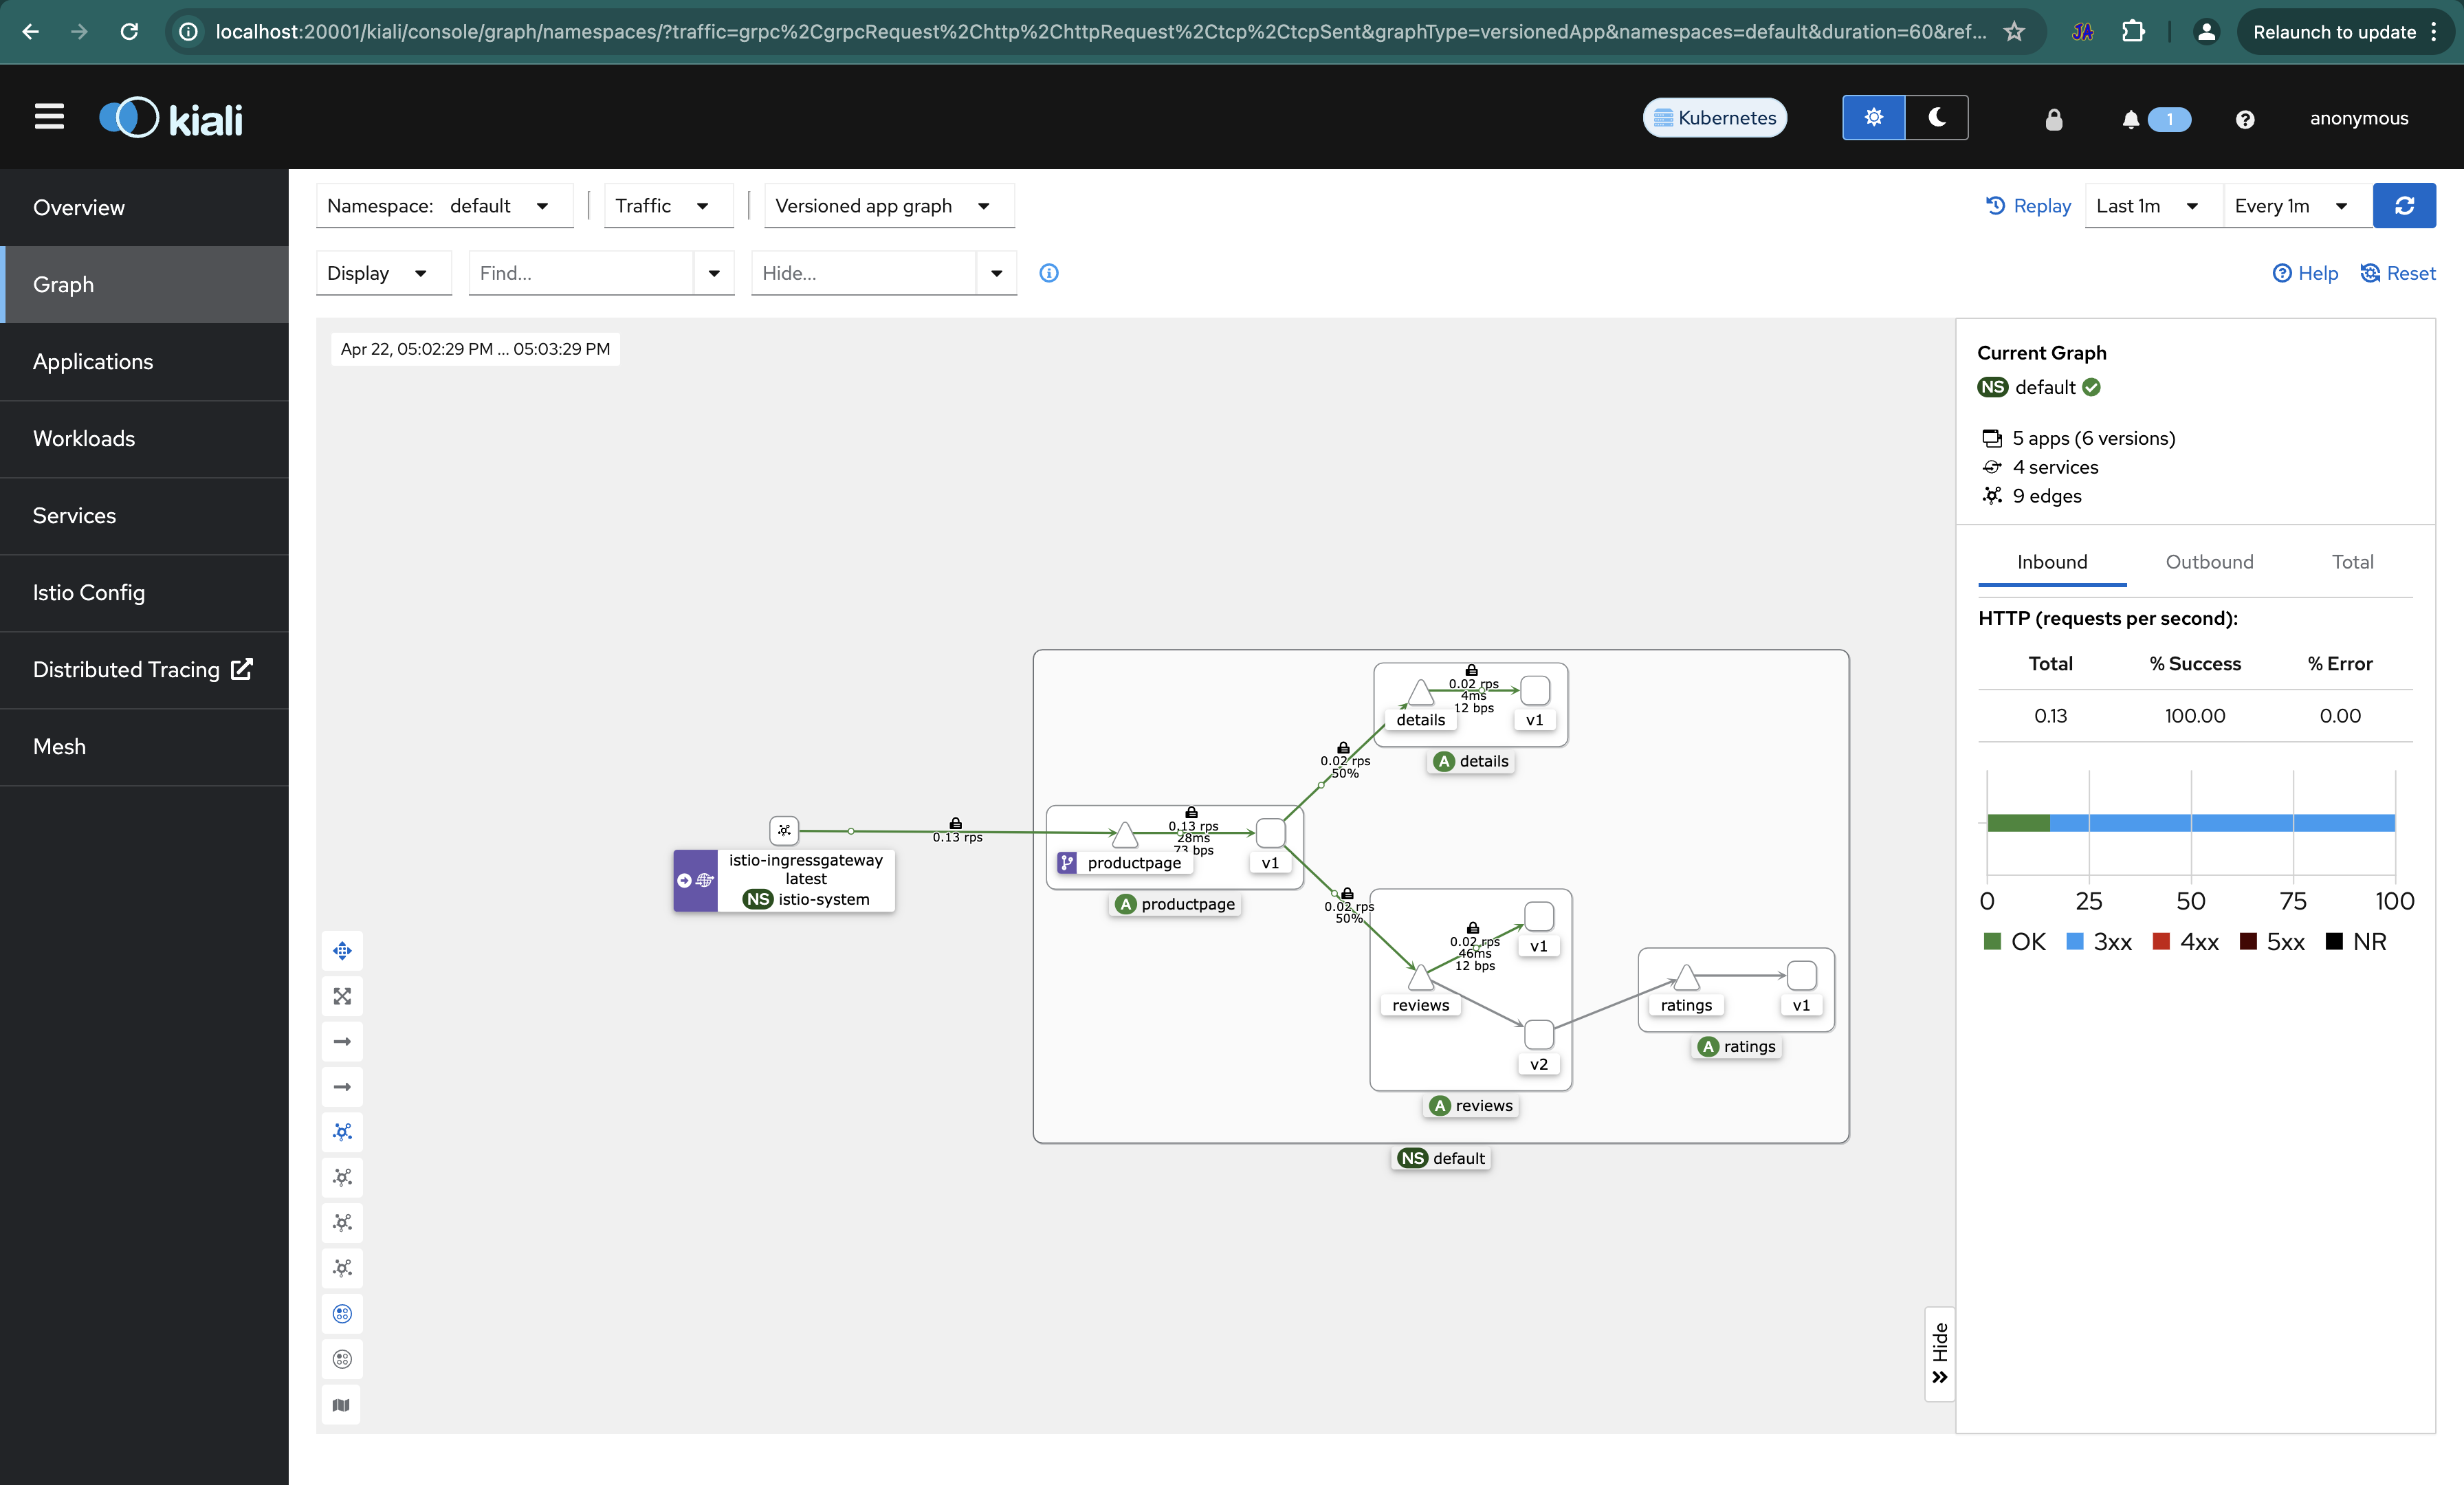
\includegraphics[width = \textwidth]{kailiConsole1.png} 
	\caption{Kaili Console} 
	\label{fig:kaili1} 
\end{figure}
\FloatBarrier



\section{Verwachte resultaten}%
\label{sec:verwachte-resultaten}

Op basis van het literatuuronderzoek vermoed ik dat het gebruik van een servicemesh een positieve impact zal hebben op de schaalbaarheid en prestatiesvan bedrijfsapplicaties. Het biedt de nodige abstractielaag en functionaliteiten om de complexe communicatie en interactie tussen microservices te beheren. Hoewel er altijd alternatieve mogelijkheden en verrassende resultaten kunnen zijn, lijkt het gebruik van een servicemesh zoals Istio een veelgebruikte en geschikte keuze te zijn op basis van de beschikbare literatuur.

%---------- Verwachte resultaten ----------------------------------------------
\section{Verwacht resultaat, conclusie}%
\label{sec:verwachte_resultaten}

Ik vermoed dat de impact van het gebruik van een servicemesh in bedrijfsapplicaties significant kan zijn. Het lijkt erop dat het gebruik van een servicemesh de mogelijkheid biedt om microservices op een schaalbare en onderhoudbare manier te beheren, wat kan resulteren in verbeterde prestaties, betere schaalbaarheid en een hogere flexibiliteit.

Er moet echter rekening worden gehouden met enkele beperkingen. Het implementeren van een servicemesh vereist waarschijnlijk een leercurve en investering in het begrijpen en toepassen van de juiste architecturale overwegingen en best practices. Daarnaast kan het beheer van een servicemesh complex zijn en extra infrastructuurkosten met zich meebrengen.

Om deze vermoedens verder te onderzoeken, zou het interessant zijn om de impact van servicemeshes in verschillende scenario's en bedrijfsomgevingen nader te onderzoeken. Het zou ook de moeite waard zijn om te onderzoeken hoe servicemeshes geoptimaliseerd kunnen worden voor specifieke gebruiksscenario's en welke aanpassingen nodig zijn om de prestaties verder te verbeteren.

Ten slotte vermoed ik dat de implementatie van een servicemesh in bedrijfsapplicaties aanzienlijke voordelen kan bieden op het gebied van schaalbaarheid, beschikaarheid, vindbaarheid en prestaties, mits de juiste architecturale overwegingen en best practices worden gevolgd. Het is weliswaar belangrijk om rekening te houden met de beperkingen en de specifieke behoeften van de applicatie en de bedrijfsdoelstellingen.

\begin{figure*}[t]   
	\centering   
	\includegraphics[width = \textwidth]{flowchart.png}  
	\caption{Flow chart}
	\label{fig:flowchart}				 
\end{figure*} 
\begin{figure*}[t]   
	\centering   
	\includegraphics[width = \textwidth]{gantt.png}   
	\caption{Gantt chart}	
	\label{fig:gantt}	
\end{figure*} 